%  sample eprint article in LaTeX           --- M. Peskin, 9/7/00
%  modified for LHCP2014, Hong Ma hma@bnl.gov
%  This file is part of a tar file, which can be downloaded from the LHCP2014 indico site. 
%    https://indico.cern.ch/event/279518/
% 


\documentclass[10pt]{article}
\usepackage{graphicx}
\usepackage{caption}
% \usepackage{subcaption}
\usepackage[subrefformat=parens,labelformat=parens]{subfig}



%%%%%%%%%%%%%%%%%%%%%%%%%%%%%%%%%%%%%%%%%%%%%%%%%%%%%%%%%%%%%%%%%%%%%%%%%%%%
%   document style macros
%%%%%%%%%%%%%%%%%%%%%%%%%%%%%%%%%%%%%%%%%%%%%%%%%%%%%%%%%%%%%%%%%%%%%%%%%%%%
\def\Title#1{\begin{center} {\Large #1 } \end{center}}
\def\Author#1{\begin{center}{ \sc #1} \end{center}}
\def\Address#1{\begin{center}{ \it #1} \end{center}}
\def\andauth{\begin{center}{and} \end{center}}
\def\submit#1{\begin{center}Submitted to {\sl #1} \end{center}}
\newcommand\pubblock{\rightline{\begin{tabular}{l} Proceedings of the Seventh Annual LHCP\\ \pubnumber\\
         \pubdate  \end{tabular}}}

\newenvironment{Abstract}{
\begin{quotation}
\begin{center} 
\large ABSTRACT \end{center}
\bigskip 
\begin{large}}
{
\end{large}
\end{quotation}
}
% \begin{center}
% \end{center}

\newenvironment{Presented}{\begin{quotation} \begin{center} 
             PRESENTED AT\end{center}\bigskip 
      \begin{center}\begin{large}}{\end{large}\end{center} \end{quotation}}

\def\Acknowledgements{\bigskip  \bigskip \begin{center} \begin{large}
             \bf ACKNOWLEDGEMENTS \end{large}\end{center}}
%%%%%%%%%%%%%%%%%%%%%%%%%%%%%%%%%%%%%%%%%%%%%%%%%%%%%%%%%%%%%%%%%%%%%%%%%%%%
%  personal abbreviations and macros
%    the following package contains macros used in this document:
\input econfmacros.tex
%%%%%%%%%%%%%%%%%%%%%%%%%%%%%%%%%%%%%%%%%%%%%%%%%%%%%%%%%%%%%%%%%%%%%%%%%%%

\textwidth=6.5in  \textheight=8.75in
\hoffset=-.85in
\voffset=-0.6in

%%  DO NOT CHANGE anything above.

% include packages you will need
\usepackage{color}

%%%%%%%%%%%%%%%%%%%%%%%%%%%%%%%%%%%%%%%%%%%%%%%%%%%%%%%%%%%%%%%%%%%%
% basic data for the eprint:
%%%%%%%%%%%%%%%%%%%%%%%%%%%%%%%%%%%%%%%%%%%%%%%%%%%%%%%%%%%%%%%%%%%%

% Instruction:
% Please change each of the following fields:
%

%% preprint number data:
% If there is a preprint number from your institute, or experiment note number, please fill it in 
\newcommand\pubnumber{ CMS-FIXME-PROC-2019-XXX }
% \newcommand\pubnumber{ }

%% date
\newcommand\pubdate{\today}

%%  Affiliation
\def\affiliation{
Department of Physics, University of California San Diego\\
9500 Gilman Drive, La Jolla, CA 92093, U.S.A }

%% Acknowledge the support
\def\support{\footnote{Work supported by  XYZ Foundation }}



\begin{document}

% large size for the first page
\large
\begin{titlepage}
\pubblock


%% Change the title, name, abstract
%% Title 
\vfill
\Title{STUDIES OF RARE ELECTROWEAK MULTIBOSON INTERACTIONS AT THE LHC}
\vfill

%  if you need to add the support use this, fill the \support definition above. 
%   \Author{ FIRSTNAME LASTNAME \support }
% \Author{ Philip Chang  }
{\begin{center}{ P. CHANG}\\
On behalf of the ATLAS and CMS Collaborations,
    \end{center}
}
% {\center
% On behalf of the ATLAS and CMS Collaborations, \\
% }
\Address{\affiliation}
\vfill
\begin{Abstract}
We present a summary of the current status of measurements in multiboson final states at the LHC from the ATLAS and CMS experiments.
Studying the rare productions of electroweak multibosons at the LHC can probe new physics beyond the energy reach of the LHC.
Various searches for rare productions of diboson and triboson are presented and their impacts to the constraints on new physics in the framework of Standard Model Effective Field Theory are also discussed.

\end{Abstract}
\vfill

% DO NOT CHANGE 
\begin{Presented}
The Seventh Annual Conference\\
 on Large Hadron Collider Physics \\
Benem\'erita Universidad Aut\'onoma de Puebla , Puebla, Mexico \\ 
May 20-25, 2019
\end{Presented}
\vfill
\end{titlepage}
\def\thefootnote{\arabic{footnote}}
\setcounter{footnote}{0}
%

% normal size for the rest
\normalsize 

%% Your paper should be entered below. 

\section{Introduction}

During Run 1 of the CERN LHC data taking, a new particle consistent with the Higgs boson of the Standard Model (SM) was discovered \cite{Aad:2012tfa,Chatrchyan:2012ufa}.
The consistency of the new particle with the SM prediction implied that there may be new physics beyond the SM (BSM) at or around the electroweak scale.
As the Run 2 of the LHC started, the collision energy was significantly increased allowing for better reach for new physics and many direct searches have been performed with the Run 2 data.
However, so far no hints of direct evidence of new physics have been seen yet\footnote{For complete exclusion summary see: https://atlas.web.cern.ch/Atlas/GROUPS/PHYSICS/CombinedSummaryPlots/ and http://cms-results.web.cern.ch/cms-results/public-results/publications/}.

The new physics could be evading our current searches for a few reasons.
The new physics may be just beyond our current constraints in which case most likely will be conformed with the Run 3 data.
It could also be that the new physics produce signatures that closely resemble known SM processes but with small rate and therefore becomes difficult in detecting.
Lastly, it is also possible that the new physics is simply beyond the energy reach of the LHC.
If the new physics is beyond the energy reach of the LHC, then it will not be possible to directly produce a new particle at the LHC.
Instead, the effects from the new physics will manifest in the data through new interactions between known SM particles \cite{Weinberg:1978kz,Weinberg:1979sa,Buchmuller:1985jz}.
This is illustrated in Figure~\subref*{fig:TailIllustration} where the new degrees of freedom from a BSM model with mass $m_{X}$ that is larger than the LHC's collision energy $E_{\tiny\textrm{LHC}}$ is integrated out leaving only the interaction between known SM fields.

\begin{figure}[htb]
\centering
    \subfloat[When $m_{X} > E_{\tiny\textrm{LHC}}$ BSM effects show up in the tails instead of as a new resonance.]{
        \label{fig:TailIllustration}
        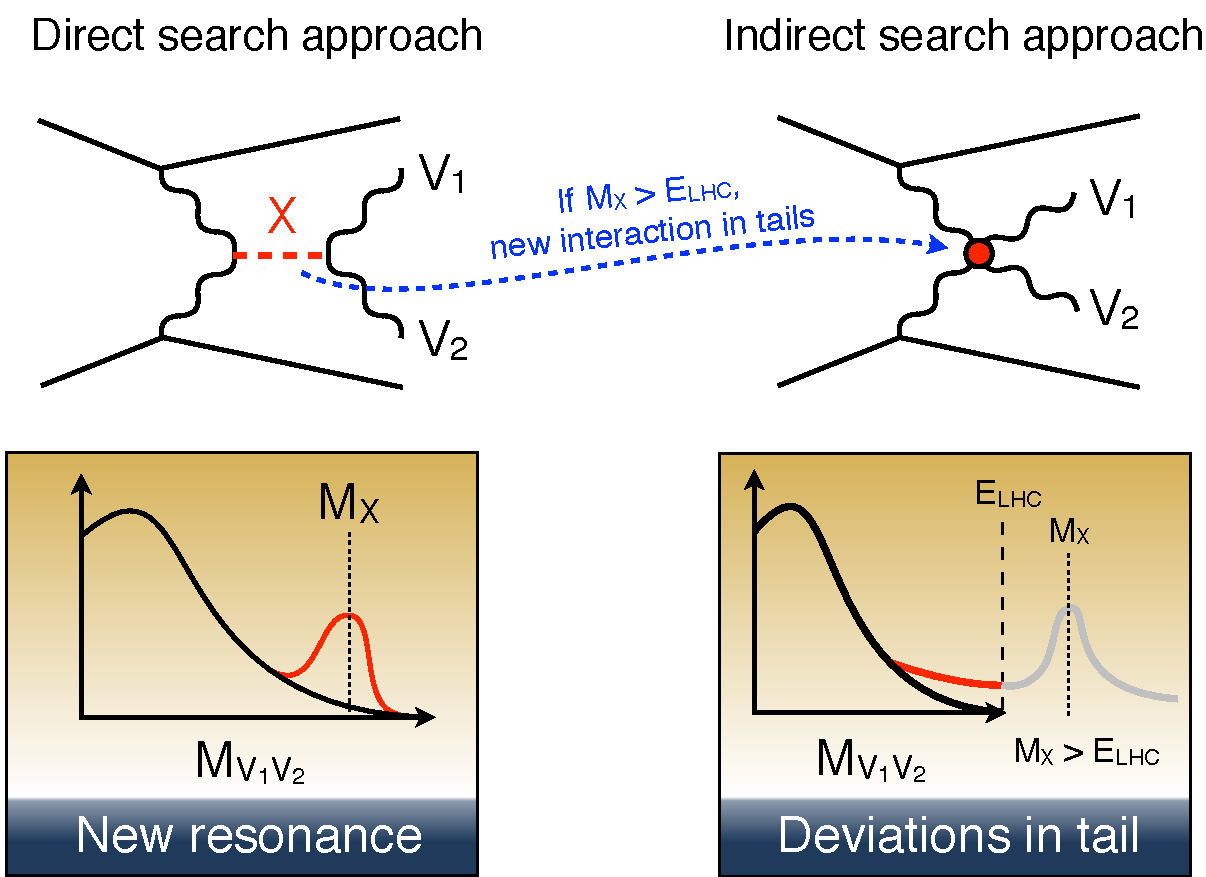
\includegraphics[height=2.4in]{TailIllustration.pdf}
        }
    \quad\quad
    \subfloat[SMEFT higher dimensional operators affecting high energy tails. Figure from \cite{Sirunyan:2019ksz} is taken to create the cartoon.]{
        \label{fig:SMEFTIllustration}
        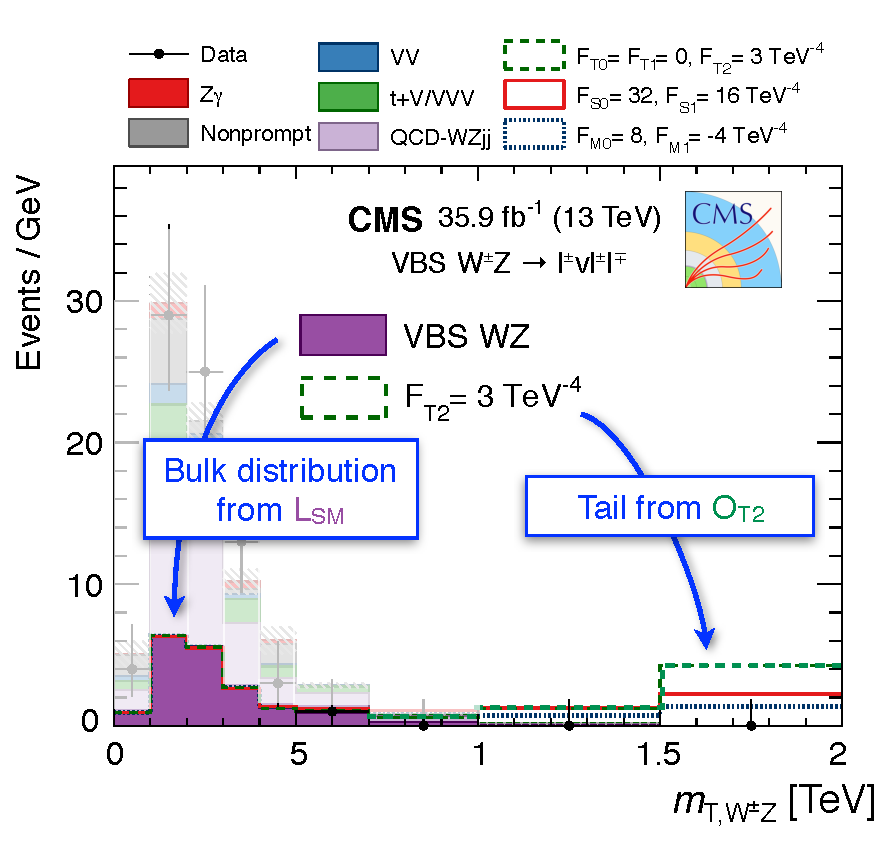
\includegraphics[height=2.4in]{SMEFTIllustration.pdf}
        }
\caption{Cartoon of BSM effects in the tails}
\label{fig:BSMTails}
\end{figure}

These possible new interactions can be systematically described by a framework called the SM Effective Field Theory (SMEFT) \cite{deBlas:2017xtg}.
In this framework, a set of higher dimensional operators constructed out of known SM fields are put together.
If there is a non-zero effect from one or some of the higher dimensional operators the effects will show up in the data as a deviation from the SM prediction.
Due to the dimensionality of these operators, the effects tend to be most pronounced in the tails of kinematic distributions, while the bulk of the kinematic distribution still roughly follows the SM prediction.
Therefore, searching for tails in kinematic distributions serve as a complementary approach to the more traditional bump hunt strategy.
It should also be noted that the bulk can also be modified by BSM models and hence measuring the bulk distribution also provides an essential confirmation of the SM.

Out of these higher dimensional operators, a handful of them predicts modifications to interactions between gauge bosons.
Therefore, SM processes involving multiboson interactions serve as an excellent testing ground to probe new physics.
As an example, a dimension-8 operator of the type,
\begin{equation}
    \mathcal{O}_{T2} = \textrm{Tr}\left[W_{\alpha\mu}W^{\mu\beta}\right]\times\textrm{Tr}\left[W_{\beta\nu}W^{\nu\alpha}\right],
\end{equation}
can lead to modifications in the distribution of the transverse mass of the $WZ$ system in the $pp\to WZjj$ process.
% increase in the tail distribution of the transverse mass of the $WZ$ system in the $pp\to WZjj$ process.
This can be seen from the Figure~\subref*{fig:SMEFTIllustration} where the modification to the $m_{T,WZ}$ distribution from the $O_{T2}$ operator is highlighted in dashed green line.
The effects are most visible in the \emph{rare} events in the tail with high energy and hence measuring the tail of such distributions can indirectly probe BSM physics.
Although not easily visible, the bulk distribution also gets modified but with a lesser degree.
Therefore, if a process at hand has a small cross section, simply observing the \emph{rare} process can also indirectly probe BSM physics.

There are many results from both ATLAS and CMS experiments related to the search or measurement of processes with multiboson interactions.
This proceeding will cover some of the recent highlights presented at the LHCP 2019.

\section{Studies of multiboson interactions in semi-leptonic final states}

In general SM processes with multiboson interactions have small cross sections due to electroweak coupling constants.
Searches with fully-leptonic decay of the $VV$ ($V=W$ or $Z$) processes, therefore, have cleaner signature with better sensitivity.
In fully-leptonic final states, often the process with the highest cross section is the signal itself, or other $VV$ processes with relatively comparable cross section.
Final states with semi-leptonic decay of the $VV$ processes, on the other hand, have SM backgrounds from $V+$jets production, which have much higher cross section, making it difficult to dig out the $VV$ signal process from the large $V+$jets background.

When considering BSM effects from higher dimensional operators, the picture changes.
Due to the smaller branching ratio of the $V$ bosons to leptonic final states, the number of expected high energy tail events for the fully-leptonic final states is significantly lower than that of the semi-leptonic final states.
In conjunction with the fact that the BSM effects can have a sizable enhancement at the tail of the distributions, studying the semi-leptonic final states can probe the BSM effects much further in the tail.
This is illustrated in Figure~\ref{fig:SemiLeptonicIllustration}.
The leptonic final states searches for rare diboson processes have already either established an observation ($>5\sigma$) or an evidence ($>3\sigma$) for the bulk distributions for various different $VV+X$ processes \cite{}.

\begin{figure}[htb]
\centering
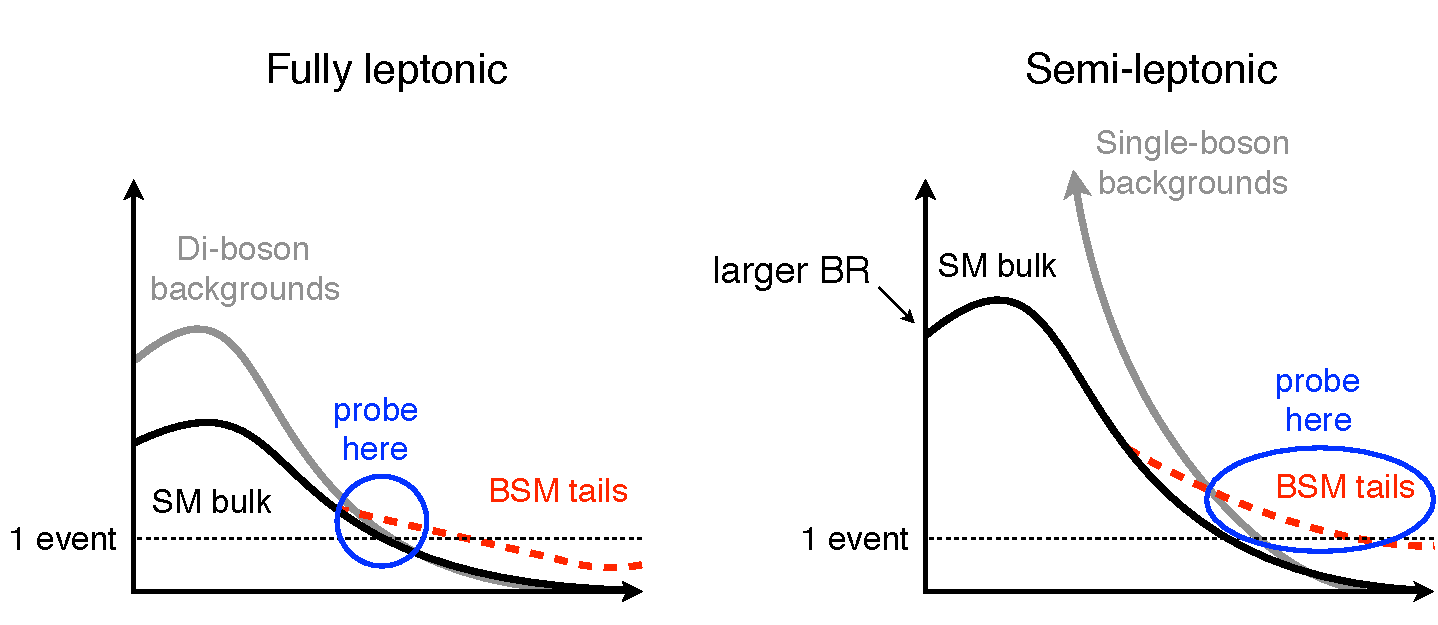
\includegraphics[height=2.0in]{SemiLeptonic.pdf}
\caption{Illustrating the complementarity between fully-leptonic and semi-leptonic final states.}
\label{fig:SemiLeptonicIllustration}
\end{figure}

\subsection{Studies of vector boson scattering processes in semi-leptonic final states}

The semi-leptonic final states searches with particular focus on the tail of the distribution have been done by the CMS experiment \cite{}.
The analysis targets signals produced via vector boson scattering (VBS).
The VBS processes have a characteristic signature where the accompanying jets (VBS jets) form a large invariant mass with a larger rapidity gap;
This search uses boosted techniques to tag the highly energetic hadronically decaying $V$ boson merging into a single fat-jet $J$.
The analysis was performed in one or two lepton final states targetting the processes such as $WV\to \ell\nu J$ or $ZV\to \ell\ell J$.
Figure~\subref*{fig:CMSVBSWV} shows the invariant mass of the $WV\to\ell\nu J$ system.
The BSM enhancement to the SM expectation is shown in the dashed line histograms.
Although the single $V+$jets processes at the bulk is very large as discussed previously, in the tail of the distribution with high invariant mass of the $WV$ system, the BSM signal has non-zero expected yields and has a rate larger than that of the $V+$jets background.
This analysis placed limits on the higher dimensional operators (specifically the dimension-8 operators) and has one of the most stringent limits to date.

Similar search has been done in ATLAS experiment as well \cite{}.
ATLAS analysis has targetted not only the tail of the distribution with merged fat-jet, but also the cases where the hadronically decaying $V$ leaves two resolved jets signature.
The analysis also targets one or two lepton final states, but in addition it also targets zero lepton final states, where it targets $ZV\to \nu\nu J$ events.
Dedicated boosted decision tree (BDT) has been trained to enhance sensitivity to the rare signal over large $V+$jets background.
Figure~\subref*{fig:ATLASVBSWV} shows the BDT distribution for the two lepton plus a fat-jet final state.
This analysis also uses novel techniques designed to separate quark vs. gluon initiated jets.
This is particularly useful as the large $V+$jets backgrounds can be accompanied by both quark or gluon initiated jets while signal process events always contain only four quark initiated jets.
The signal regions are split into 9 different regions and the respective BDT distribution in each regions are fitted simultaneously to extract the signal.
The observed and expected sensitivity is 2.7$\sigma$ and 2.5$\sigma$ respectively.

\begin{figure}[htb]
\centering
    \subfloat[]{
        \label{fig:CMSVBSWV}
        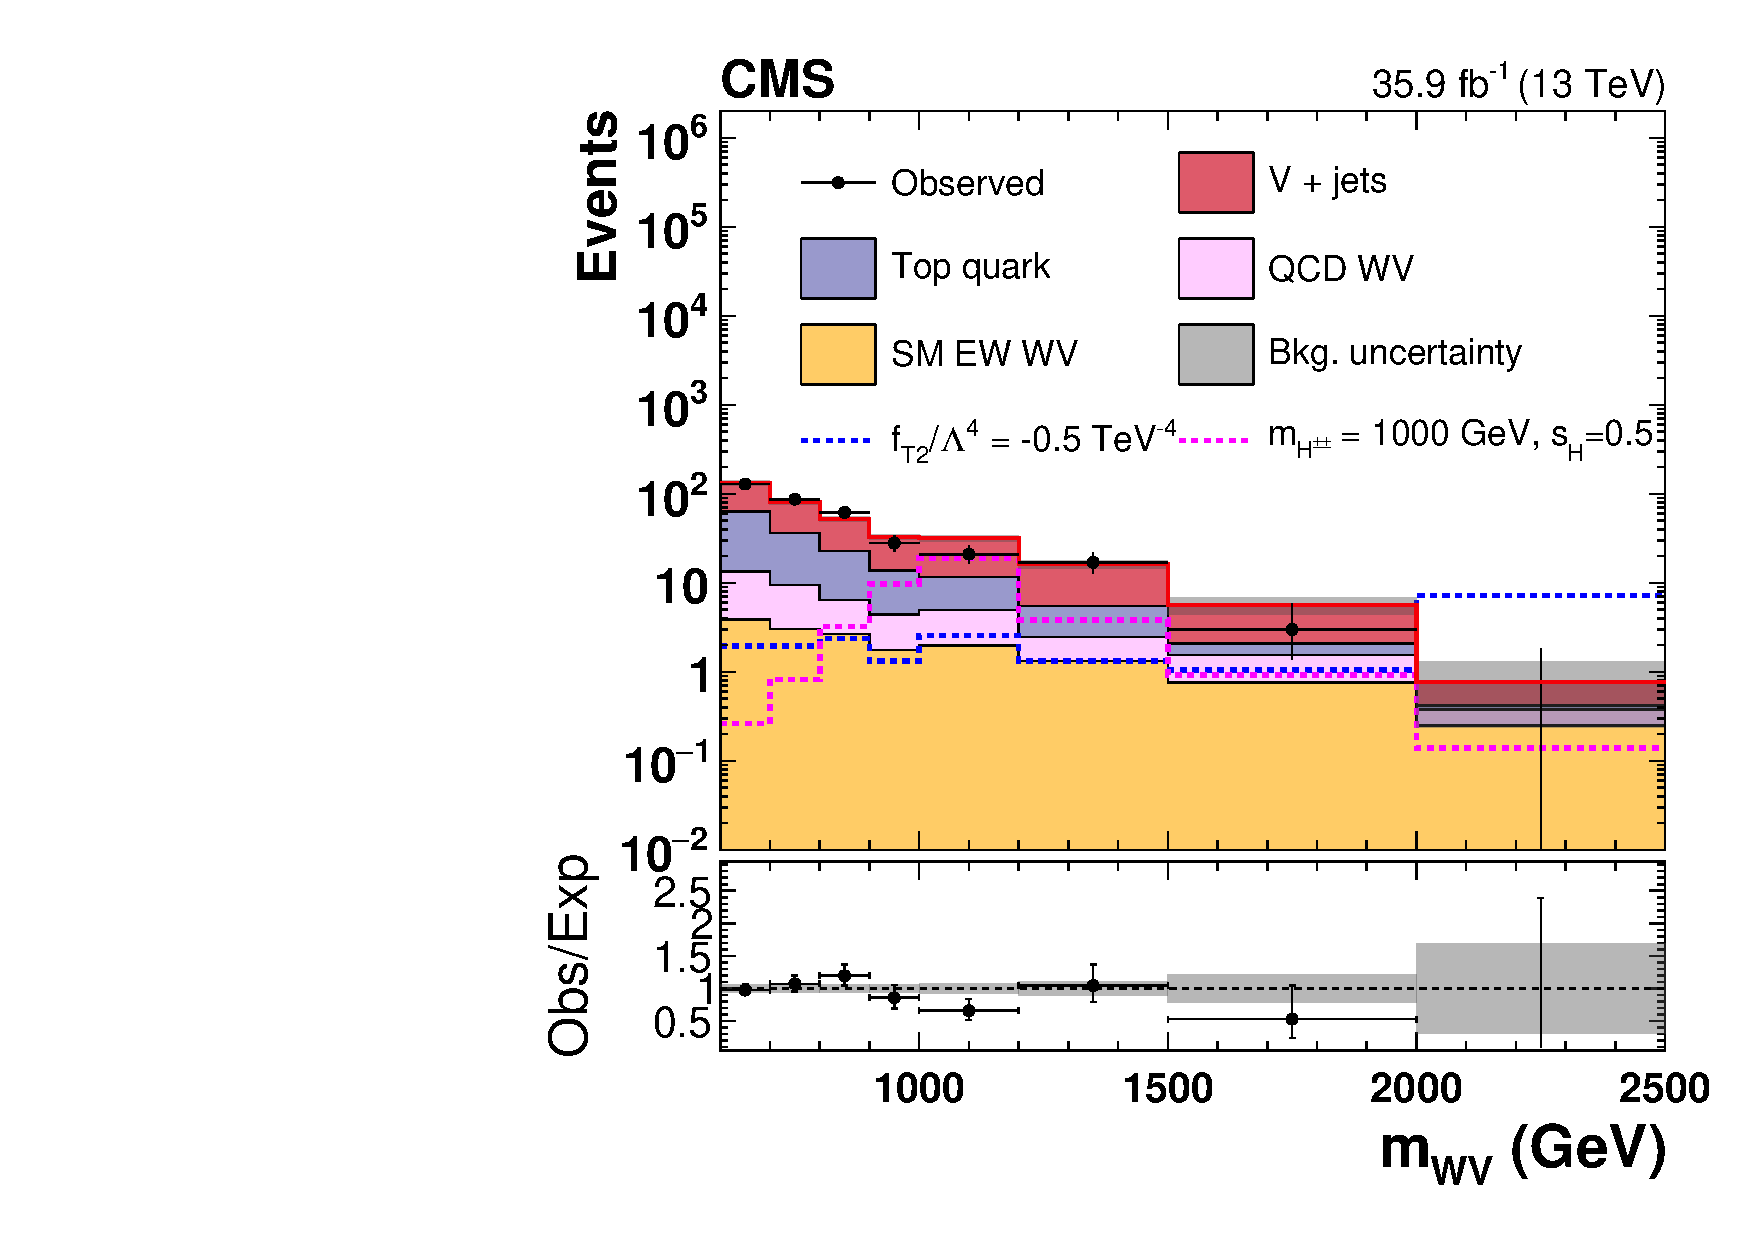
\includegraphics[height=2.4in]{CMS-SMP-18-006_Figure_004-a.pdf}
        }
    \quad\quad
    \subfloat[]{
        \label{fig:ATLASVBSWV}
        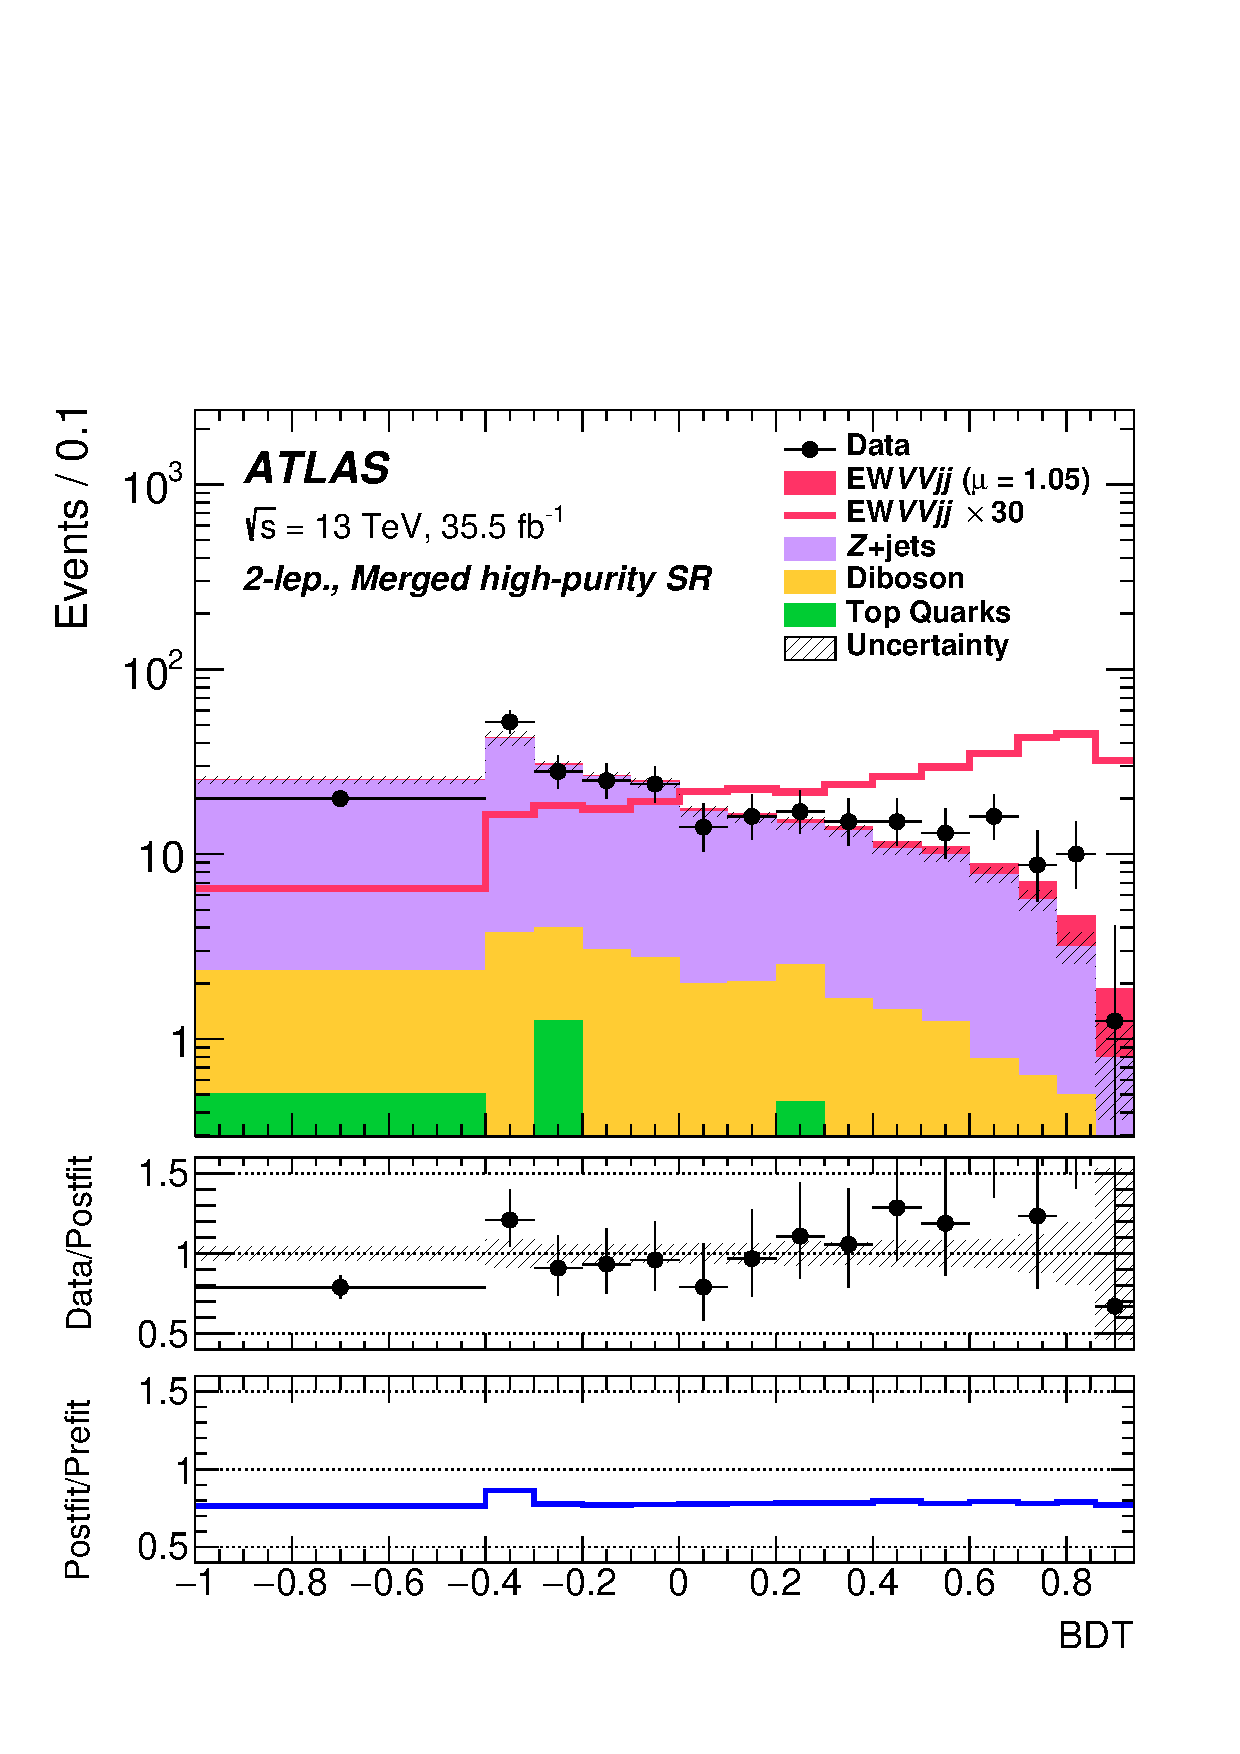
\includegraphics[height=2.4in]{fig_06a.pdf}
        }
\caption{Cartoon of BSM effects in the tails}
\label{fig:BSMTails}
\end{figure}

\subsection{Studies of diboson processes in semi-leptonic final states}
\label{sec:CMSWV}

CMS experiment also performed a search in semi-leptonic final states of diboson production involving triple gauge couplings (TGCs).
The signal process is $pp\to VV$ without any VBS jets.
The analysis also utilizes boosted techniques to tag the merged fat-jet from a hadronically decaying $V$ boson.
Figure~\subref*{fig:CMSWV} shows the invariant mass distribution of the $pp\to WV\to e\nu J$ system.
Although the actual $pp\to WV$ process is well below the very large $W+$jets background process, starting around $m_{WV} > 2.5$~TeV the BSM effects from the higher dimensional operators become dominant over the $W+$jets.
Both the signal and the background distributions are parametrized using a series of exponential function and fitted simultaneously to extract limits on the dimension-6 operators (viz. $\mathcal{O}_{WWW}$, $\mathcal{O}_{W}$, and $\mathcal{O}_{B}$).
The analysis is not sensitive to the SM rate of the $WV$ boson over a large $W+$jets background but places the most stringent limits on some of the dimension-6 operators to date.
The limits to the coefficients of the dimension-6 operators (represented as $c_{i} / \Lambda^2$) are shown in Table~\ref{tab:CMSWVLimits}.
Deviations from zero indicate new physics, and the result is consistent with the SM.

\begin{figure}[htb]
\centering
    \subfloat[]{
        \label{fig:CMSWV}
        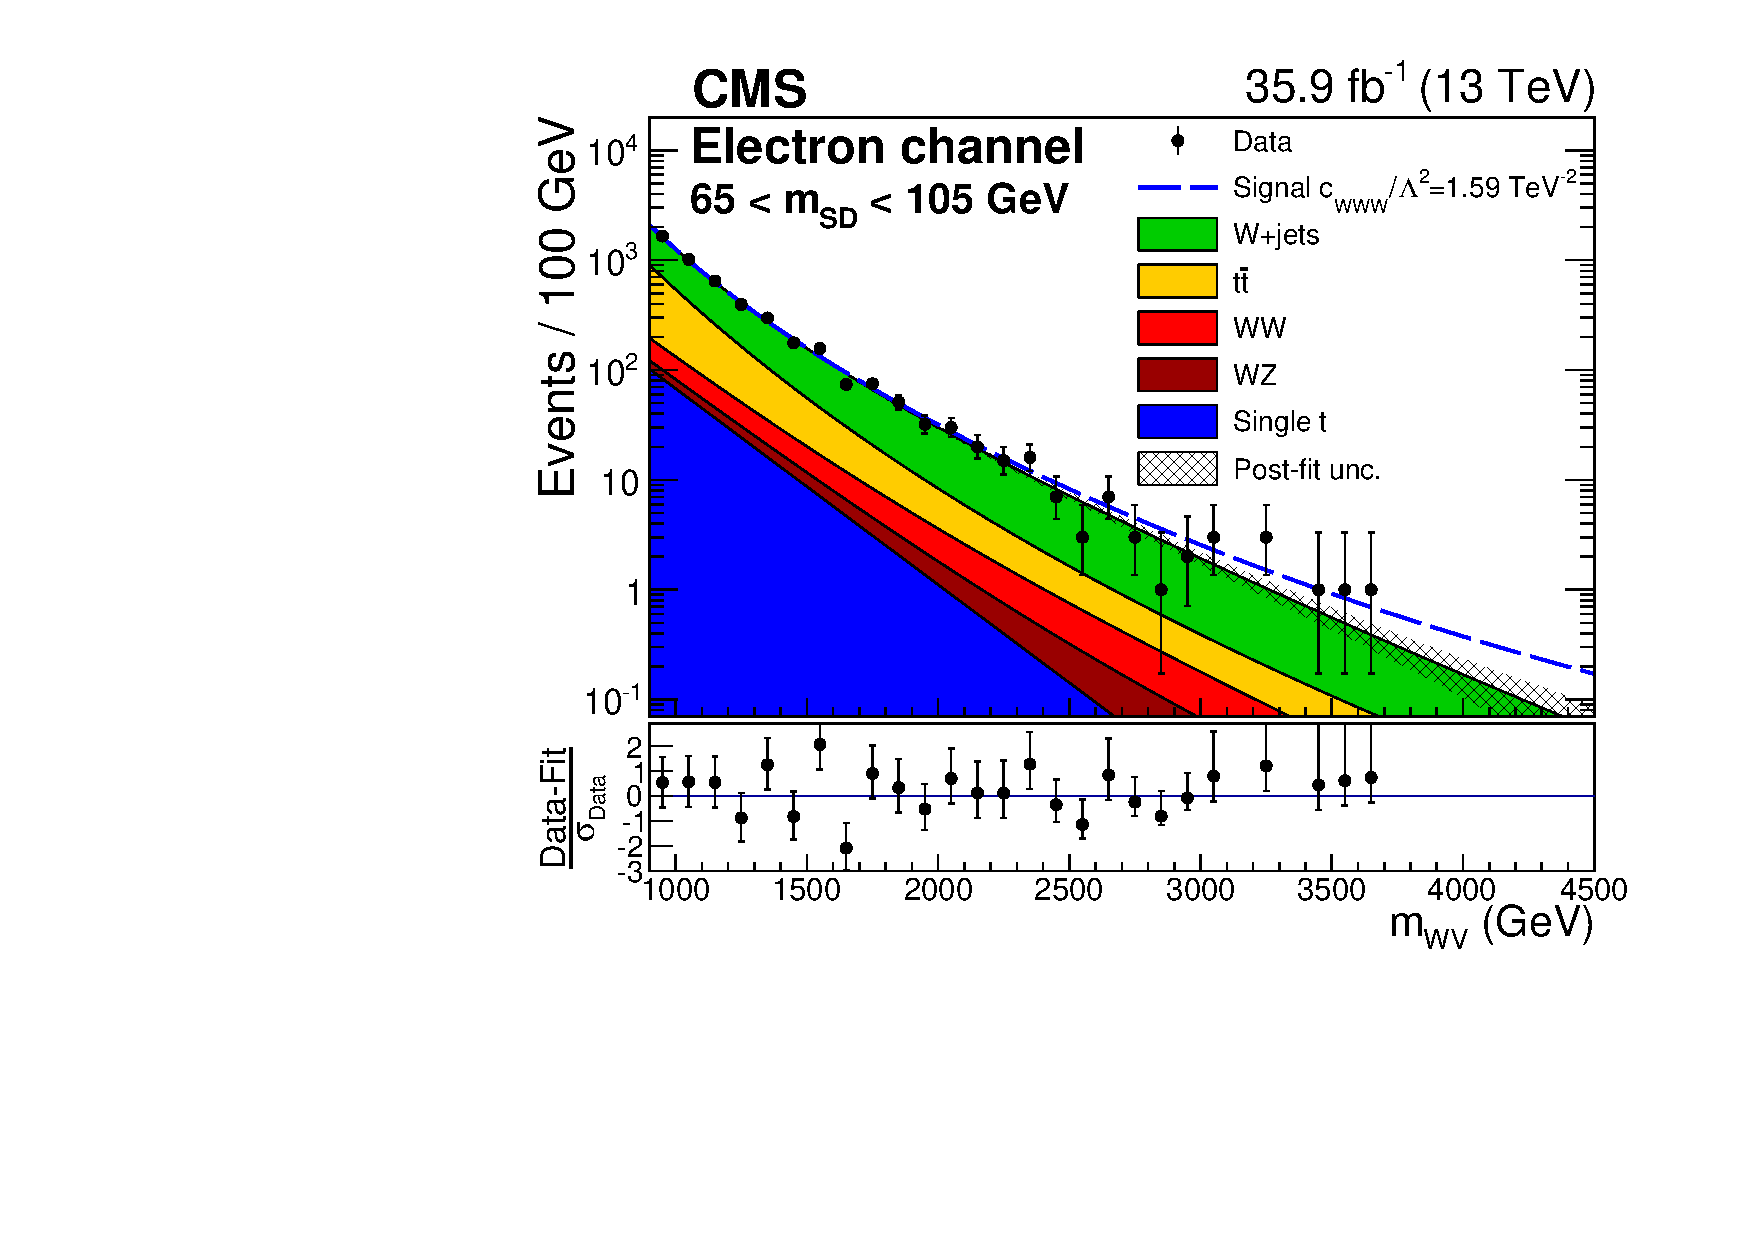
\includegraphics[height=2.2in]{CMS-SMP-18-008_Figure_004-c.pdf}
        }
    \quad\quad
    \subfloat[]{
        \label{fig:VBFWPtl}
        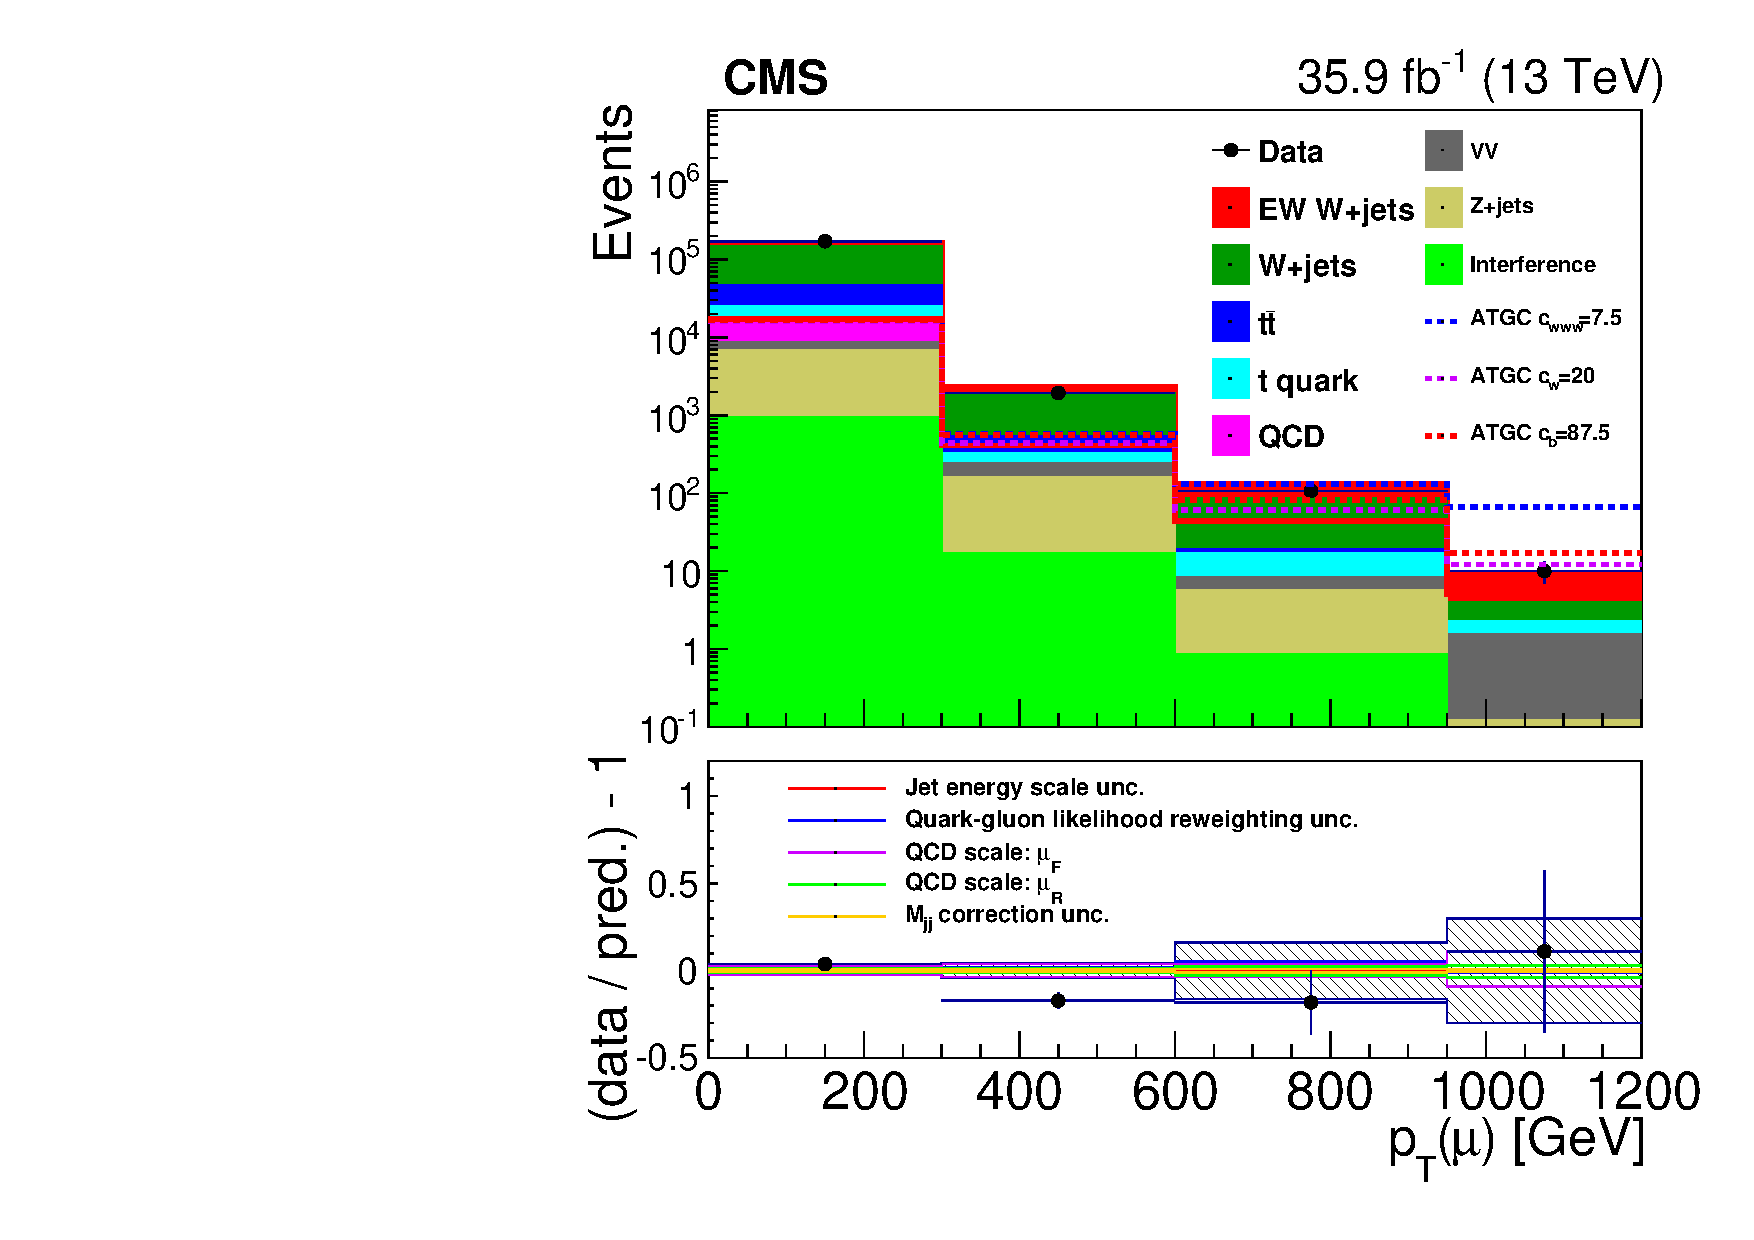
\includegraphics[height=2.2in]{CMS-SMP-17-011_Figure_010-a.pdf}
        }
\caption{}
\label{fig:BSMTails}
\end{figure}

\begin{table}[t]
\begin{center}
\caption{}
\label{tab:CMSWVLimits}
\begin{tabular}{l|ccc}  
Operator coefficients & Expected limit & Observed limit & Observed best-fit \\ \hline
$c_{WWW} / \Lambda^2$ & [-1.44,1.47]   & [-1.58,1.59]   & -0.26  \\
$c_{W} / \Lambda^2$   & [-2.45,2.08]   & [-2.00,2.65]   & 1.21   \\
$c_{B} / \Lambda^2$   & [-8.38,8.06]   & [-8.78,8.54]   & 1.07   \\
\end{tabular}
\end{center}
\end{table}

\subsection{Single $W$ production via vector boson fusion}

Contrary to na\"ive expectation, the process $pp \to W jj$ involves multiboson interactions.
The Feynman diagram is the same as the process studied in the Section~\ref{sec:CMSWV} except through crossing.
The production of single $W$ boson occurs through fusion of the two $V$ bosons radiated from the incoming partons and hence is called vector boson fusion (VBF).
The accompanying jets (VBF jets) from the process also exhibits the same characteristics as the VBS jets.

CMS has performed an analysis targetting $pp \to W jj$.
A multivariate discriminant is trained using BDT method.
This analysis also utilizes quark-gluon tagging technique in order to separate $W+$jets background from signal where the signal's VBF jets are always quark initiated jets.
The final BDT discriminant is fitted to extract the signal.
The analysis has established the signal with well over $>5\sigma$ significance.
The analysis then bins the events by the transverse momentum of the leptons $p_{T,\ell}$ and extract limits on dimension-6 operators.
Figure~\subref*{fig:VBFWPtl} shows the distribution of the $p_{T,\ell}$.
The effects from the dimension-6 operators are shown at the tail of the distribution as expected.
The limits to the dimension-6 operators are shown in Table~\ref{tab:CMSVBFWLimits}.
In the case for the dimension-6 operators $\mathcal{O}_{WWW}$, the constraint is weaker but comparable to the $pp \to WV$ analysis presented in Section~\ref{sec:CMSWV}, demonstrating complementarity between the two analyses.

\begin{table}[t]
\begin{center}
\caption{ place the caption here }
\label{tab:CMSVBFWLimits}
\begin{tabular}{l|cc}  
Operator coefficients & Expected limit & Observed limit\\ \hline
$c_{WWW} / \Lambda^2$ & [-2.5,2.5]     & [-2.3,2.5]    \\
$c_{W} / \Lambda^2$   & [-16,19]       & [-8.8,1.6]    \\
$c_{B} / \Lambda^2$   & [-62,61]       & [-45,46]      \\
\end{tabular}
\end{center}
\end{table}
\subsection{Triboson production}



% Slide 12
Triboson

% Slide 13
WWW

% Slide 14 / 15
WWZ/ZZZ

% Future













%\section{Observations}

%REPLACE THE TEXT, FIGURE and TABLE.

%Observation of the Higgs Boson,  \cite{Aad:2012tfa},\cite{Chatrchyan:2012ufa}. 

 
%%%%%%%%%%%%%%%%%%%%%%%%%%%%%%%%%%%%%%%%%%%%%%%%%%%%%%%%%%%%%%%%%%%%%%%%%%
%%%
%%%   use this format to include an .eps figure into your paper
%%%
%\begin{figure}[htb]
%\centering
%% 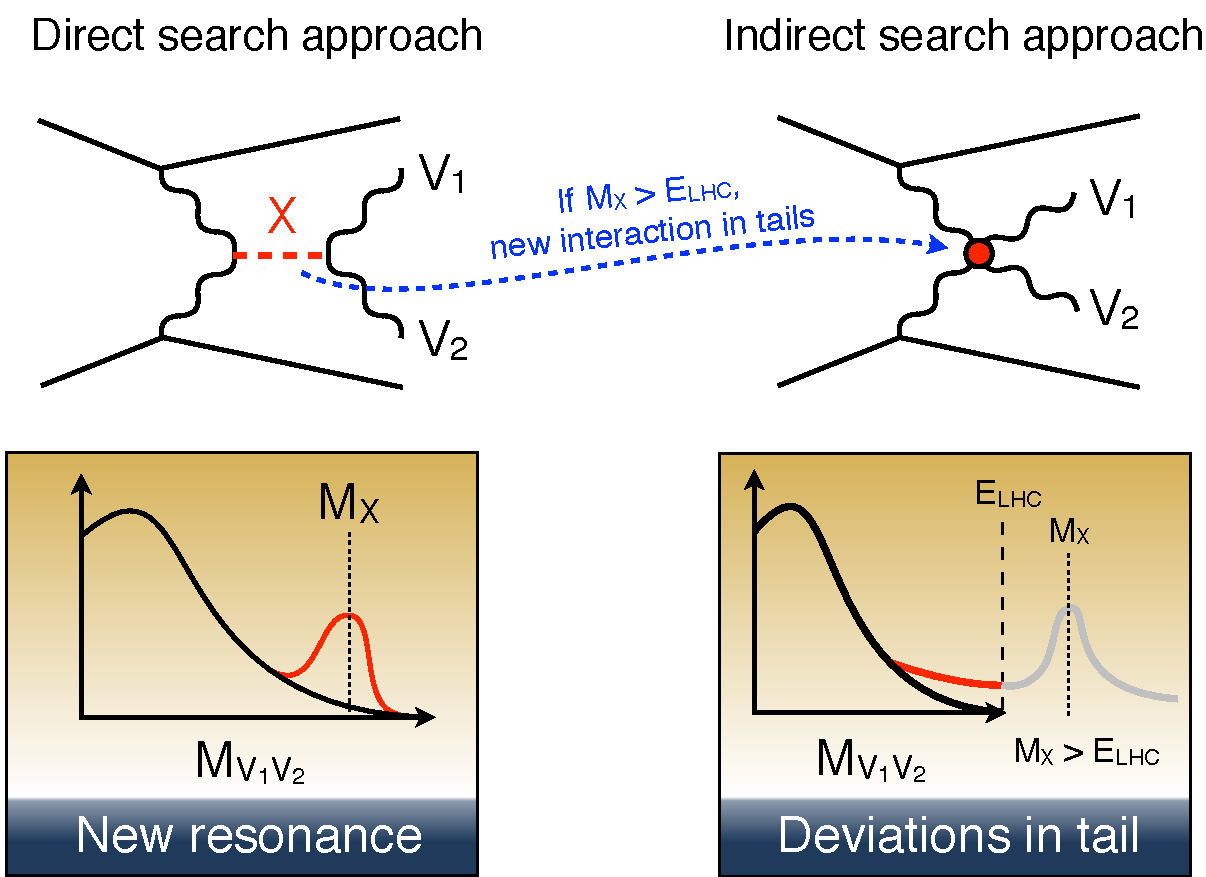
\includegraphics[height=2in]{TailIllustration.pdf}
%\caption{ Place the caption here}
%\label{fig:figure1}
%\end{figure}
%%%%%%%%%%%%%%%%%%%%%%%%%%%%%%%%%%%%%%%%%%%%%%%%%%%%%%%%%%%%%%%%%%%%%%%%%%%%

%See Figure \ref{fig:figure1} and Table \ref{tab:table1}. 

%%%%%%%%%%%%%%%%%%%%%%%%%%%%%%%%%%%%%%%%%%%%%%%%%%%%%%%%%%%%%%%%%%%%%%%%%%
%%%
%%%   use this format to include a LaTeX table  into your paper
%%%
%\begin{table}[t]
%\begin{center}
%\begin{tabular}{l|ccc}  
%Patient &  Initial level($\mu$g/cc) &  w. Magnet &  
%w. Magnet and Sound \\ \hline
% Guglielmo B.  &   0.12     &     0.10      &     0.001  \\
% Ferrando di N. &  0.15     &     0.11      &  $< 0.0005$ \\ \hline
%\end{tabular}
%\caption{ place the caption here }
%\label{tab:table1}
%\end{center}
%\end{table}
%%%%%%%%%%%%%%%%%%%%%%%%%%%%%%%%%%%%%%%%%%%%%%%%%%%%%%%%%%%%%%%%%%%%%%%%%%%%

%\section{Interpretations}

%The conference banquet will be hosted at the Spirit of New York, dinner while on a three-hour cruise around Manhattan. Enjoy an evening of most entertaining and unique combination of dining, dancing, entertainment and views on New York Harbor. Registered attendees and accompanying guests are invited to attend. 


\section{Conclusions}

...... 

%%  if necessary
\Acknowledgements
I am grateful to XYZ for fruitful discussions.


\begin{thebibliography}{99}

%%
%%  bibliographic items can be constructed using the LaTeX format in SPIRES:
%%    see    http://www.slac.stanford.edu/spires/hep/latex.html
%%  SPIRES will also supply the CITATION line information; please include it.
%%

\bibitem{Aad:2012tfa} 
  G.~Aad {\it et al.}  [ATLAS Collaboration],
  %``Observation of a new particle in the search for the Standard Model Higgs boson with the ATLAS detector at the LHC,''
  Phys.\ Lett.\ B {\bf 716}, 1 (2012)
  [arXiv:1207.7214 [hep-ex]].
  %%CITATION = ARXIV:1207.7214;%%
  %3009 citations counted in INSPIRE as of 22 Jul 2014
  
  
%\cite{Chatrchyan:2012ufa}
\bibitem{Chatrchyan:2012ufa} 
  S.~Chatrchyan {\it et al.}  [CMS Collaboration],
  %``Observation of a new boson at a mass of 125 GeV with the CMS experiment at the LHC,''
  Phys.\ Lett.\ B {\bf 716}, 30 (2012)
  [arXiv:1207.7235 [hep-ex]].
  %%CITATION = ARXIV:1207.7235;%%
  %2951 citations counted in INSPIRE as of 22 Jul 2014

%\cite{Weinberg:1978kz}
\bibitem{Weinberg:1978kz} 
  S.~Weinberg,
  %``Phenomenological Lagrangians,''
  Physica A {\bf 96}, no. 1-2, 327 (1979).
  doi:10.1016/0378-4371(79)90223-1
  %%CITATION = doi:10.1016/0378-4371(79)90223-1;%%
  %3256 citations counted in INSPIRE as of 16 Aug 2019

%\cite{Weinberg:1979sa}
\bibitem{Weinberg:1979sa} 
  S.~Weinberg,
  %``Baryon and Lepton Nonconserving Processes,''
  Phys.\ Rev.\ Lett.\  {\bf 43}, 1566 (1979).
  doi:10.1103/PhysRevLett.43.1566
  %%CITATION = doi:10.1103/PhysRevLett.43.1566;%%
  %1561 citations counted in INSPIRE as of 15 Aug 2019

%\cite{Buchmuller:1985jz}
\bibitem{Buchmuller:1985jz} 
  W.~Buchmuller and D.~Wyler,
  %``Effective Lagrangian Analysis of New Interactions and Flavor Conservation,''
  Nucl.\ Phys.\ B {\bf 268}, 621 (1986).
  doi:10.1016/0550-3213(86)90262-2
  %%CITATION = doi:10.1016/0550-3213(86)90262-2;%%
  %1563 citations counted in INSPIRE as of 15 Aug 2019

%\cite{Sirunyan:2019ksz}
\bibitem{Sirunyan:2019ksz} 
  A.~M.~Sirunyan {\it et al.} [CMS Collaboration],
  %``Measurement of electroweak WZ boson production and search for new physics in WZ + two jets events in pp collisions at $\sqrt{s} =$ 13TeV,''
  Phys.\ Lett.\ B {\bf 795}, 281 (2019)
  doi:10.1016/j.physletb.2019.05.042
  [arXiv:1901.04060 [hep-ex]].
  %%CITATION = doi:10.1016/j.physletb.2019.05.042;%%
  %7 citations counted in INSPIRE as of 16 Aug 2019

%\cite{deBlas:2017xtg}
\bibitem{deBlas:2017xtg} 
  J.~de Blas, J.~C.~Criado, M.~Perez-Victoria and J.~Santiago,
  %``Effective description of general extensions of the Standard Model: the complete tree-level dictionary,''
  JHEP {\bf 1803}, 109 (2018)
  doi:10.1007/JHEP03(2018)109
  [arXiv:1711.10391 [hep-ph]].
  %%CITATION = doi:10.1007/JHEP03(2018)109;%%
  %33 citations counted in INSPIRE as of 16 Aug 2019


\end{thebibliography}

 
\end{document}

% The bulk distribution is also slightly modified is also highlighted in Figure~\ref{fig:SMEFTIllustration} in purple.
% In conclusion there are two checks one can do, 

% Figure~\ref{fig:SMEFTIllustration} illustrates how measuring the \emph{rare} events with multiboson interactions in the tail of the kinematic distributions can constrain new physics indirectly.
% Moreover, if a process at hand already has a small cross section, simply observing the rare events with multiboson interactions

% These new interactions manifest as higher dimensional operators constructed out of the SM fields.
% The number of higher dimensional operators constructed out of SM fields can easily reach the thousands, but a subset of higher dimensional operators that are of interest have been put together in the framework called the SM Effective Field Theory (SMEFT)\cite{}.
% It is worth noting that the 

% If the higher dimensional operators have a non-zero coefficient the effects from them will show up in

% The new interactions tend to be most visible at kinematic distributions with high energy and therefore is more easily detectable at the tails of kinematic distributions.

% While the bulk distribution is governed by the SM predictions as usual, the \emph{rare} tail events 

% Slide 4
% The SM processes involving multiboson interactions tend to be low in cross section.
% The couplings between gauge bosons are fully determined by the non-Abelian structure of the SM theory, namely the $SU(2)_\mathrm{L}\times U(1)_{Y}$.


% Studies of multiboson interactions serve as an excellent testing ground for various higher dimensional operators.

% As an example the Figure shows an effect from the operator of the following blah blah 

% VBS WW
@article{Aad:2014zda,
      author         = "Aad, Georges and others",
      title          = "{Evidence for Electroweak Production of
                        $W^{\pm}W^{\pm}jj$ in $pp$ Collisions at $\sqrt{s}=8$ TeV
                        with the ATLAS Detector}",
      collaboration  = "ATLAS",
      journal        = "Phys. Rev. Lett.",
      volume         = "113",
      year           = "2014",
      number         = "14",
      pages          = "141803",
      doi            = "10.1103/PhysRevLett.113.141803",
      eprint         = "1405.6241",
      archivePrefix  = "arXiv",
      primaryClass   = "hep-ex",
      reportNumber   = "CERN-PH-EP-2014-079",
      SLACcitation   = "%%CITATION = ARXIV:1405.6241;%%"
}

@article{Aaboud:2019nmv,
      author         = "Aaboud, Morad and others",
      title          = "{Observation of electroweak production of a same-sign $W$
                        boson pair in association with two jets in $pp$ collisions
                        at $\sqrt{s}=13$ TeV with the ATLAS detector}",
      collaboration  = "ATLAS",
      year           = "2019",
      eprint         = "1906.03203",
      archivePrefix  = "arXiv",
      primaryClass   = "hep-ex",
      reportNumber   = "CERN-EP-2019-008",
      SLACcitation   = "%%CITATION = ARXIV:1906.03203;%%"
}

@article{Khachatryan:2014sta,
      author         = "Khachatryan, Vardan and others",
      title          = "{Study of vector boson scattering and search for new
                        physics in events with two same-sign leptons and two
                        jets}",
      collaboration  = "CMS",
      journal        = "Phys. Rev. Lett.",
      volume         = "114",
      year           = "2015",
      number         = "5",
      pages          = "051801",
      doi            = "10.1103/PhysRevLett.114.051801",
      eprint         = "1410.6315",
      archivePrefix  = "arXiv",
      primaryClass   = "hep-ex",
      reportNumber   = "CMS-SMP-13-015, CERN-PH-EP-2014-250",
      SLACcitation   = "%%CITATION = ARXIV:1410.6315;%%"
}

@article{Sirunyan:2017ret,
      author         = "Sirunyan, Albert M and others",
      title          = "{Observation of electroweak production of same-sign W
                        boson pairs in the two jet and two same-sign lepton final
                        state in proton-proton collisions at $\sqrt{s} = $ 13
                        TeV}",
      collaboration  = "CMS",
      journal        = "Phys. Rev. Lett.",
      volume         = "120",
      year           = "2018",
      number         = "8",
      pages          = "081801",
      doi            = "10.1103/PhysRevLett.120.081801",
      eprint         = "1709.05822",
      archivePrefix  = "arXiv",
      primaryClass   = "hep-ex",
      reportNumber   = "CMS-SMP-17-004, CERN-EP-2017-232",
      SLACcitation   = "%%CITATION = ARXIV:1709.05822;%%"
}

% VBS WZ
@article{Aad:2016ett,
      author         = "Aad, Georges and others",
      title          = "{Measurements of $W^\pm Z$ production cross sections in
                        $pp$ collisions at $\sqrt{s} = 8$ TeV with the ATLAS
                        detector and limits on anomalous gauge boson
                        self-couplings}",
      collaboration  = "ATLAS",
      journal        = "Phys. Rev.",
      volume         = "D93",
      year           = "2016",
      number         = "9",
      pages          = "092004",
      doi            = "10.1103/PhysRevD.93.092004",
      eprint         = "1603.02151",
      archivePrefix  = "arXiv",
      primaryClass   = "hep-ex",
      reportNumber   = "CERN-EP-2016-017",
      SLACcitation   = "%%CITATION = ARXIV:1603.02151;%%"
}

@article{Aaboud:2018ddq,
      author         = "Aaboud, Morad and others",
      title          = "{Observation of electroweak $W^{\pm}Z$ boson pair
                        production in association with two jets in $pp$ collisions
                        at $\sqrt{s} =$ 13 TeV with the ATLAS detector}",
      collaboration  = "ATLAS",
      journal        = "Phys. Lett.",
      volume         = "B793",
      year           = "2019",
      pages          = "469-492",
      doi            = "10.1016/j.physletb.2019.05.012",
      eprint         = "1812.09740",
      archivePrefix  = "arXiv",
      primaryClass   = "hep-ex",
      reportNumber   = "CERN-EP-2018-286",
      SLACcitation   = "%%CITATION = ARXIV:1812.09740;%%"
}

@article{Sirunyan:2019ksz,
      author         = "Sirunyan, Albert M and others",
      title          = "{Measurement of electroweak WZ boson production and
                        search for new physics in WZ + two jets events in pp
                        collisions at $\sqrt{s} =$ 13TeV}",
      collaboration  = "CMS",
      journal        = "Phys. Lett.",
      volume         = "B795",
      year           = "2019",
      pages          = "281-307",
      doi            = "10.1016/j.physletb.2019.05.042",
      eprint         = "1901.04060",
      archivePrefix  = "arXiv",
      primaryClass   = "hep-ex",
      reportNumber   = "CMS-SMP-18-001, CERN-EP-2018-333",
      SLACcitation   = "%%CITATION = ARXIV:1901.04060;%%"
}
